% Options for packages loaded elsewhere
\PassOptionsToPackage{unicode}{hyperref}
\PassOptionsToPackage{hyphens}{url}
%
\documentclass[
  ignorenonframetext,
  aspectratio=169]{beamer}
\usepackage{pgfpages}
\setbeamertemplate{caption}[numbered]
\setbeamertemplate{caption label separator}{: }
\setbeamercolor{caption name}{fg=normal text.fg}
\beamertemplatenavigationsymbolsempty
% Prevent slide breaks in the middle of a paragraph
\widowpenalties 1 10000
\raggedbottom
\setbeamertemplate{part page}{
  \centering
  \begin{beamercolorbox}[sep=16pt,center]{part title}
    \usebeamerfont{part title}\insertpart\par
  \end{beamercolorbox}
}
\setbeamertemplate{section page}{
  \centering
  \begin{beamercolorbox}[sep=12pt,center]{part title}
    \usebeamerfont{section title}\insertsection\par
  \end{beamercolorbox}
}
\setbeamertemplate{subsection page}{
  \centering
  \begin{beamercolorbox}[sep=8pt,center]{part title}
    \usebeamerfont{subsection title}\insertsubsection\par
  \end{beamercolorbox}
}
\AtBeginPart{
  \frame{\partpage}
}
\AtBeginSection{
  \ifbibliography
  \else
    \frame{\sectionpage}
  \fi
}
\AtBeginSubsection{
  \frame{\subsectionpage}
}
\usepackage{amsmath,amssymb}
\usepackage{iftex}
\ifPDFTeX
  \usepackage[T1]{fontenc}
  \usepackage[utf8]{inputenc}
  \usepackage{textcomp} % provide euro and other symbols
\else % if luatex or xetex
  \usepackage{unicode-math} % this also loads fontspec
  \defaultfontfeatures{Scale=MatchLowercase}
  \defaultfontfeatures[\rmfamily]{Ligatures=TeX,Scale=1}
\fi
\usepackage{lmodern}
\ifPDFTeX\else
  % xetex/luatex font selection
\fi
% Use upquote if available, for straight quotes in verbatim environments
\IfFileExists{upquote.sty}{\usepackage{upquote}}{}
\IfFileExists{microtype.sty}{% use microtype if available
  \usepackage[]{microtype}
  \UseMicrotypeSet[protrusion]{basicmath} % disable protrusion for tt fonts
}{}
\makeatletter
\@ifundefined{KOMAClassName}{% if non-KOMA class
  \IfFileExists{parskip.sty}{%
    \usepackage{parskip}
  }{% else
    \setlength{\parindent}{0pt}
    \setlength{\parskip}{6pt plus 2pt minus 1pt}}
}{% if KOMA class
  \KOMAoptions{parskip=half}}
\makeatother
\usepackage{xcolor}
\newif\ifbibliography
\usepackage{color}
\usepackage{fancyvrb}
\newcommand{\VerbBar}{|}
\newcommand{\VERB}{\Verb[commandchars=\\\{\}]}
\DefineVerbatimEnvironment{Highlighting}{Verbatim}{commandchars=\\\{\}}
% Add ',fontsize=\small' for more characters per line
\usepackage{framed}
\definecolor{shadecolor}{RGB}{248,248,248}
\newenvironment{Shaded}{\begin{snugshade}}{\end{snugshade}}
\newcommand{\AlertTok}[1]{\textcolor[rgb]{0.94,0.16,0.16}{#1}}
\newcommand{\AnnotationTok}[1]{\textcolor[rgb]{0.56,0.35,0.01}{\textbf{\textit{#1}}}}
\newcommand{\AttributeTok}[1]{\textcolor[rgb]{0.13,0.29,0.53}{#1}}
\newcommand{\BaseNTok}[1]{\textcolor[rgb]{0.00,0.00,0.81}{#1}}
\newcommand{\BuiltInTok}[1]{#1}
\newcommand{\CharTok}[1]{\textcolor[rgb]{0.31,0.60,0.02}{#1}}
\newcommand{\CommentTok}[1]{\textcolor[rgb]{0.56,0.35,0.01}{\textit{#1}}}
\newcommand{\CommentVarTok}[1]{\textcolor[rgb]{0.56,0.35,0.01}{\textbf{\textit{#1}}}}
\newcommand{\ConstantTok}[1]{\textcolor[rgb]{0.56,0.35,0.01}{#1}}
\newcommand{\ControlFlowTok}[1]{\textcolor[rgb]{0.13,0.29,0.53}{\textbf{#1}}}
\newcommand{\DataTypeTok}[1]{\textcolor[rgb]{0.13,0.29,0.53}{#1}}
\newcommand{\DecValTok}[1]{\textcolor[rgb]{0.00,0.00,0.81}{#1}}
\newcommand{\DocumentationTok}[1]{\textcolor[rgb]{0.56,0.35,0.01}{\textbf{\textit{#1}}}}
\newcommand{\ErrorTok}[1]{\textcolor[rgb]{0.64,0.00,0.00}{\textbf{#1}}}
\newcommand{\ExtensionTok}[1]{#1}
\newcommand{\FloatTok}[1]{\textcolor[rgb]{0.00,0.00,0.81}{#1}}
\newcommand{\FunctionTok}[1]{\textcolor[rgb]{0.13,0.29,0.53}{\textbf{#1}}}
\newcommand{\ImportTok}[1]{#1}
\newcommand{\InformationTok}[1]{\textcolor[rgb]{0.56,0.35,0.01}{\textbf{\textit{#1}}}}
\newcommand{\KeywordTok}[1]{\textcolor[rgb]{0.13,0.29,0.53}{\textbf{#1}}}
\newcommand{\NormalTok}[1]{#1}
\newcommand{\OperatorTok}[1]{\textcolor[rgb]{0.81,0.36,0.00}{\textbf{#1}}}
\newcommand{\OtherTok}[1]{\textcolor[rgb]{0.56,0.35,0.01}{#1}}
\newcommand{\PreprocessorTok}[1]{\textcolor[rgb]{0.56,0.35,0.01}{\textit{#1}}}
\newcommand{\RegionMarkerTok}[1]{#1}
\newcommand{\SpecialCharTok}[1]{\textcolor[rgb]{0.81,0.36,0.00}{\textbf{#1}}}
\newcommand{\SpecialStringTok}[1]{\textcolor[rgb]{0.31,0.60,0.02}{#1}}
\newcommand{\StringTok}[1]{\textcolor[rgb]{0.31,0.60,0.02}{#1}}
\newcommand{\VariableTok}[1]{\textcolor[rgb]{0.00,0.00,0.00}{#1}}
\newcommand{\VerbatimStringTok}[1]{\textcolor[rgb]{0.31,0.60,0.02}{#1}}
\newcommand{\WarningTok}[1]{\textcolor[rgb]{0.56,0.35,0.01}{\textbf{\textit{#1}}}}
\usepackage{longtable,booktabs,array}
\usepackage{calc} % for calculating minipage widths
\usepackage{caption}
% Make caption package work with longtable
\makeatletter
\def\fnum@table{\tablename~\thetable}
\makeatother
\usepackage{graphicx}
\makeatletter
\def\maxwidth{\ifdim\Gin@nat@width>\linewidth\linewidth\else\Gin@nat@width\fi}
\def\maxheight{\ifdim\Gin@nat@height>\textheight\textheight\else\Gin@nat@height\fi}
\makeatother
% Scale images if necessary, so that they will not overflow the page
% margins by default, and it is still possible to overwrite the defaults
% using explicit options in \includegraphics[width, height, ...]{}
\setkeys{Gin}{width=\maxwidth,height=\maxheight,keepaspectratio}
% Set default figure placement to htbp
\makeatletter
\def\fps@figure{htbp}
\makeatother
\setlength{\emergencystretch}{3em} % prevent overfull lines
\providecommand{\tightlist}{%
  \setlength{\itemsep}{0pt}\setlength{\parskip}{0pt}}
\setcounter{secnumdepth}{-\maxdimen} % remove section numbering
\usetheme{Goettingen}
\renewcommand{\textbf}{\structure}
\renewcommand{\mathbf}{\structure}
\addtobeamertemplate{navigation symbols}{}{ \usebeamerfont{footline} }
\addtobeamertemplate{navigation symbols}{}{ \usebeamercolor[fg]{footline} }
\addtobeamertemplate{navigation symbols}{}{ \insertframenumber/\inserttotalframenumber }
\usepackage[os=win]{menukeys}
\usepackage{soul}
\usepackage{xcolor}
\usepackage{caption}
\usepackage[os=win]{menukeys}
\usepackage{copyrightbox}
\ifLuaTeX
  \usepackage{selnolig}  % disable illegal ligatures
\fi
\IfFileExists{bookmark.sty}{\usepackage{bookmark}}{\usepackage{hyperref}}
\IfFileExists{xurl.sty}{\usepackage{xurl}}{} % add URL line breaks if available
\urlstyle{same}
\hypersetup{
  pdftitle={Lecture 36: Non-parametric statistical tests},
  hidelinks,
  pdfcreator={LaTeX via pandoc}}

\title{Lecture 36: Non-parametric statistical tests}
\subtitle{Nov 27, 2023 (Slides by Corinne Riddell)}
\author{}
\date{\vspace{-2.5em}}

\begin{document}
\frame{\titlepage}

\begin{frame}
\end{frame}

\begin{frame}{Concussions}
\protect\hypertarget{concussions}{}
\begin{center}
\includegraphics[width=0.5\linewidth]{./images/concussionmovie} \end{center}
\end{frame}

\begin{frame}{Concussions: NY times April 10,2019}
\protect\hypertarget{concussions-ny-times-april-102019}{}
\begin{center}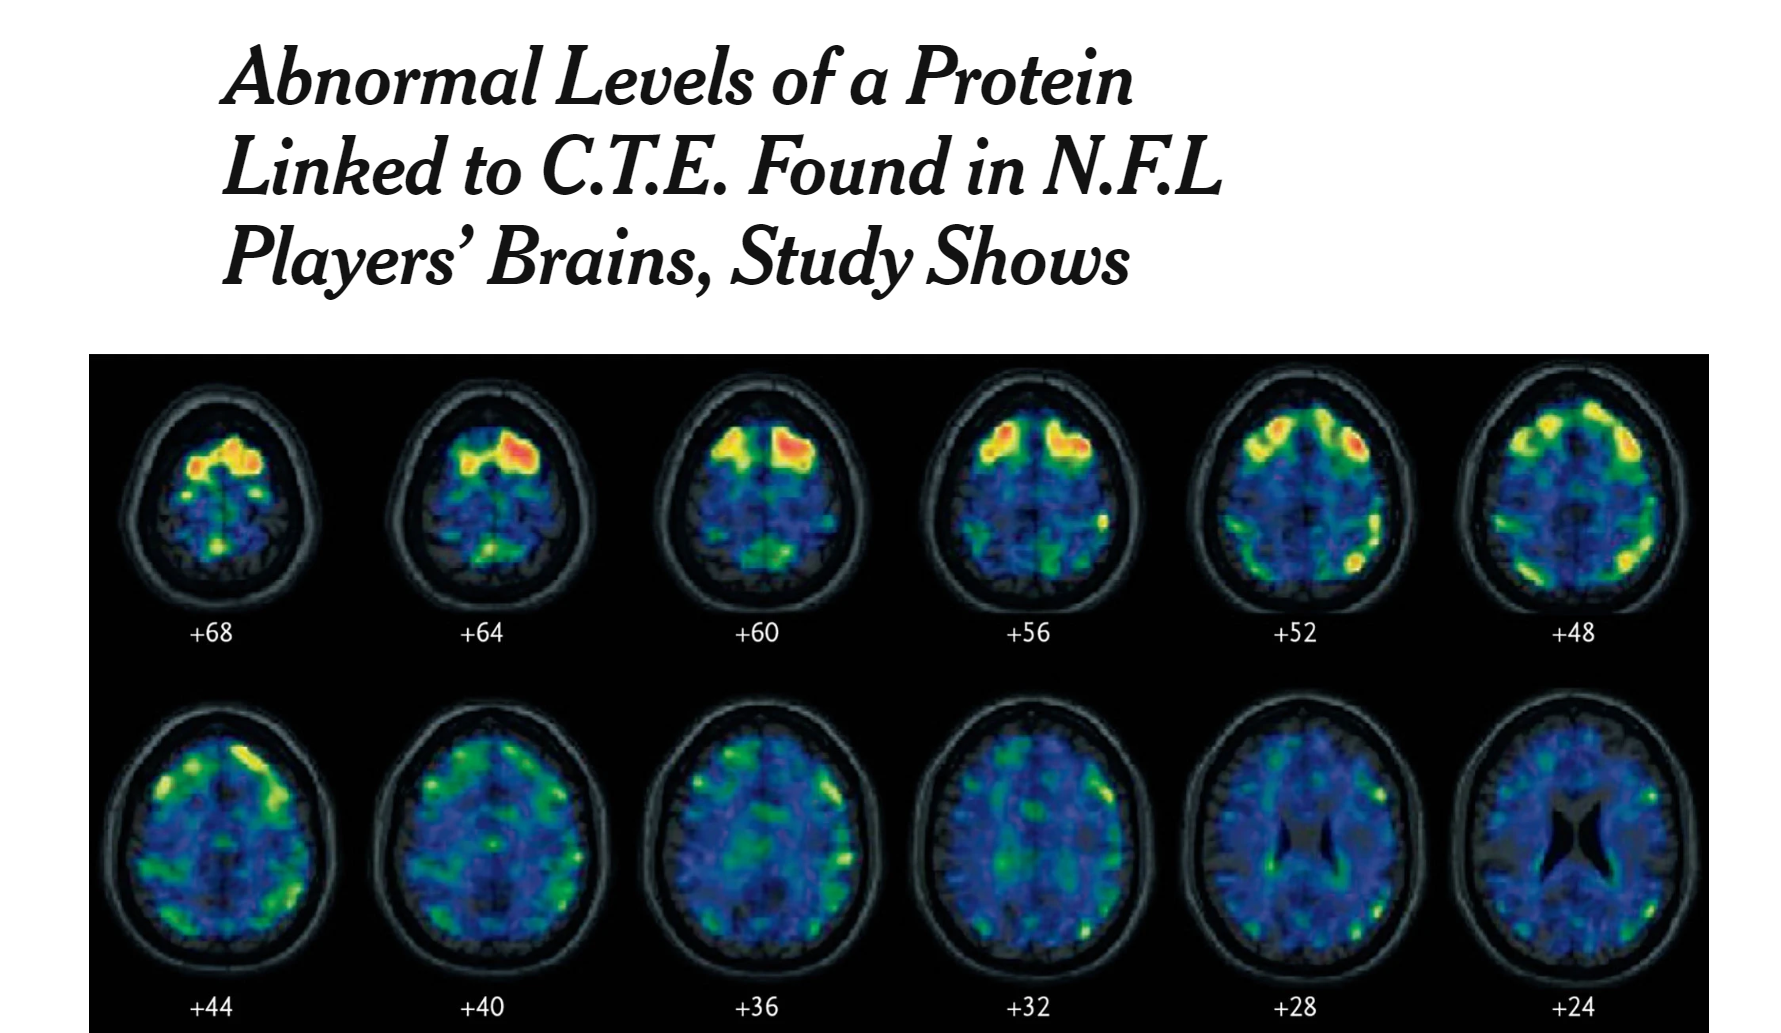
\includegraphics[width=0.8\linewidth]{./images/concussion_nytimes} \end{center}

\href{https://www.nytimes.com/2019/04/10/health/concussion-nfl-football-cte.html}{NYtimes
article}
\end{frame}

\begin{frame}{From the article}
\protect\hypertarget{from-the-article}{}
\begin{center}
\includegraphics[width=0.7\linewidth]{./images/concussion_nejm} \end{center}

The authors of the study and outside experts stressed that such tau
imaging is far from a diagnostic test for C.T.E., which is likely years
away and could include other markers, from blood and spinal fluid.

The results of the study, published in The New England Journal of
Medicine on Wednesday, are considered preliminary, but constitute a
first step toward developing a clinical test to determine the presence
of C.T.E. in living players, as well as early signs and potential risk.
\end{frame}

\begin{frame}{From the article}
\protect\hypertarget{from-the-article-1}{}
STATISTICAL ANALYSIS Between-group comparisons of age, years of
education, and MMSE scores were analyzed with \textbf{Mann--Whitney U
tests}. Group differences in race were analyzed with the use of
chi-square tests. For between-group comparisons of amyloid-beta plaque
burden, chi-square tests were used to compare the proportion of
participants with a positive florbetapir PET, and \textbf{t-tests} were
used to compare the mean cortical:cerebellar florbetapir standard uptake
value ratio (SUVR, the ratio of radioactivity in a cerebral region to
that in the cerebellum as a reference) between the groups.
\end{frame}

\begin{frame}{From the article}
\protect\hypertarget{from-the-article-2}{}
\begin{center}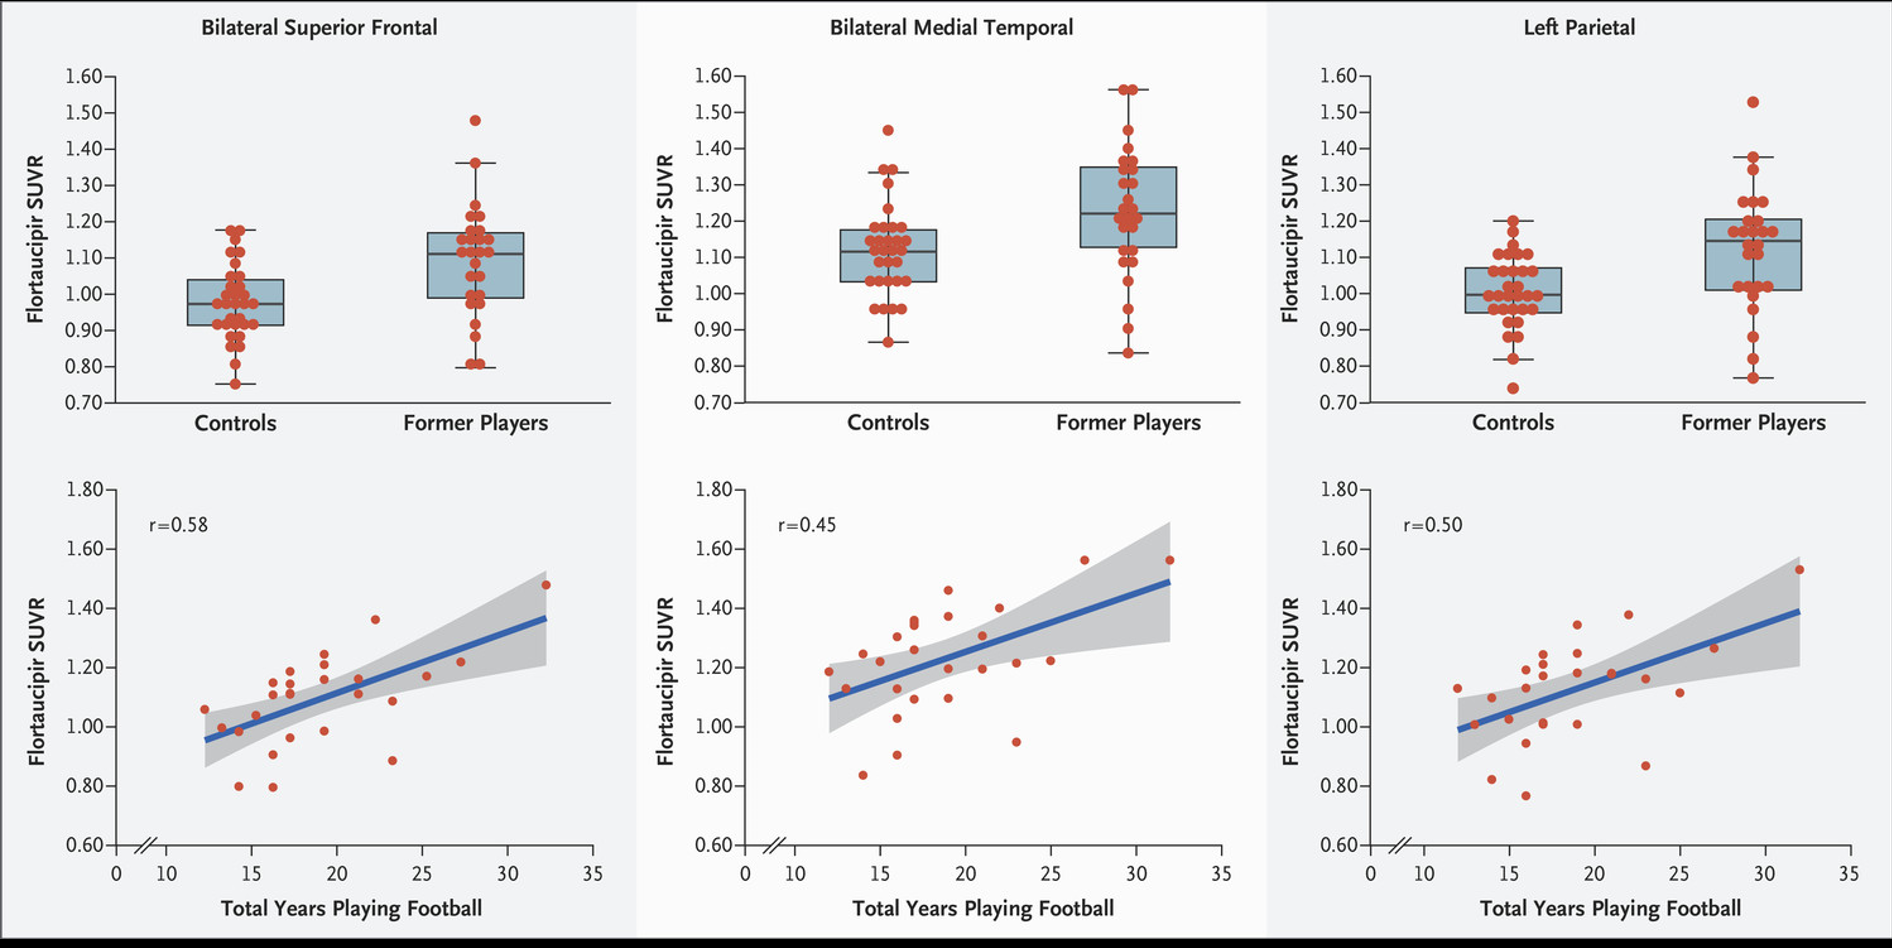
\includegraphics[width=0.7\linewidth]{./images/concussion_graphs} \end{center}
\end{frame}

\begin{frame}{Roadmap}
\protect\hypertarget{roadmap}{}
In part II :

\begin{itemize}
\tightlist
\item
  One sample comparison to a mean (one sample t)
\item
  Two independent samples (two sample t)
\item
  Two non-independent samples (paired t)
\item
  Multiple samples/groups (ANOVA)

  \begin{itemize}
  \tightlist
  \item
    Bonferroni
  \item
    Tukey's HSD
  \end{itemize}
\end{itemize}
\end{frame}

\begin{frame}{Roadmap}
\protect\hypertarget{roadmap-1}{}
But all of the methods we have looked at so far depend on some
assumptions about the underlying distribution.

What have we assumed?

What do we do if our assumptions are violated?
\end{frame}

\hypertarget{non-parametric-testing}{%
\subsection{Non-Parametric testing}\label{non-parametric-testing}}

\begin{frame}{Non-Parametric Testing}
\protect\hypertarget{non-parametric-testing-1}{}
From \url{http://biostatisticsryangoslingreturns.tumblr.com/}

\begin{center}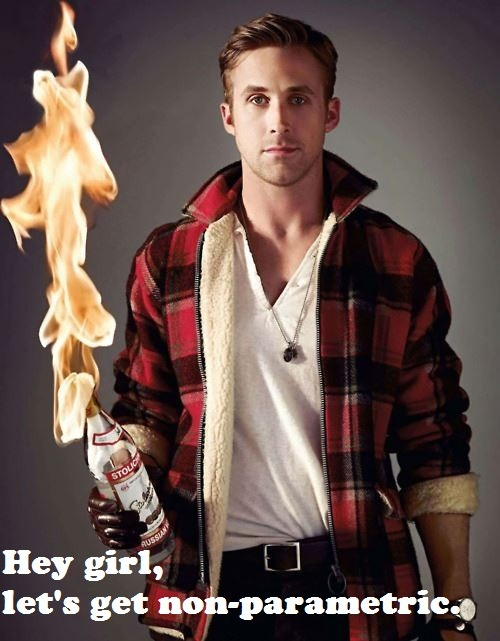
\includegraphics[width=0.6\linewidth]{./images/nonpara} \end{center}
\end{frame}

\begin{frame}{Non-Parametric Testing}
\protect\hypertarget{non-parametric-testing-2}{}
\textbf{PROS}: Non-parametric methods make very few assumptions about
the variable(s) we samples or their distribution and thus rely less on
``parameters''.

\begin{itemize}
\tightlist
\item
  Use a ranking of the data instead of actual values
\item
  Do not assume a normal distribution of the data
\item
  Less sensitive to outliers and skewed data
\item
  Do not need a large sample size (sometimes)
\end{itemize}

\textbf{CONS}: Non-parametric methods use less of the information
offered in the data

\begin{itemize}
\tightlist
\item
  If the assumptions of for a parametric test are met and a
  non-parametric test is used, it will have lower power (probability of
  detecting a false null hypothesis)
\item
  They are less specific in what they test (e.g., independence)
\end{itemize}
\end{frame}

\begin{frame}{Non-Parametric Testing}
\protect\hypertarget{non-parametric-testing-3}{}
We will discuss non-parametric equivalents for:

Two sample t : Wilcoxon Rank-Sum

Paired t : Wilcoxon sign-rank

ANOVA: Kruskal Wallis
\end{frame}

\hypertarget{wilcoxon-two-sample-tests}{%
\subsection{Wilcoxon two-sample tests}\label{wilcoxon-two-sample-tests}}

\begin{frame}{Frank Wilcoxon}
\protect\hypertarget{frank-wilcoxon}{}
\begin{center}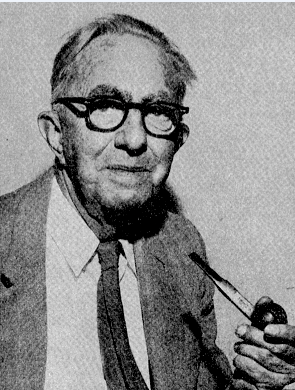
\includegraphics[width=0.6\linewidth]{./images/wilcox} \end{center}

In one paper in 1945 he proposed both the Wilcoxon rank-sum test and the
Wilcoxon signed-rank test
\end{frame}

\begin{frame}{Wilcoxon Rank-Sum}
\protect\hypertarget{wilcoxon-rank-sum}{}
\begin{itemize}
\tightlist
\item
  Sometimes also called the Mann-Whitney U test
\item
  Non-parametric test for comparing two independent samples with a
  continuous outcome
\item
  This is the non-parametric counterpart of the two sample t-test
\item
  Assumes that the distributions have the same general shape but assumes
  nothing about that shape.\\
\item
  Evaluates the null hypothesis that the two population distributions
  are identical.
\end{itemize}
\end{frame}

\begin{frame}{Wilcoxon Rank-Sum}
\protect\hypertarget{wilcoxon-rank-sum-1}{}
To calculate a rank sum test

The observations are ordered from lowest to highest and assigned the
\textbf{rank} of their order.

If there are ``tie'' values, these are assigned the average of the
ranks, ie if two observations have the same value and the next lower
value is rank=3 then the two observations are both given the rank of 4.5
(because they would have been ranks 4 and 5).

Then the sums of ranks belonging to group 1 are compared to the sums of
ranks belonging to group 2
\end{frame}

\begin{frame}{Wilcoxon Rank-Sum}
\protect\hypertarget{wilcoxon-rank-sum-2}{}
Values in group 1: 4,3,5,2,6

Values in group 2: 6,5,7,4,8
\end{frame}

\begin{frame}{Wilcoxon Rank-Sum}
\protect\hypertarget{wilcoxon-rank-sum-3}{}
\begin{longtable}[]{@{}llll@{}}
\toprule\noalign{}
Group 1 & rank & Group 2 & rank \\
\midrule\noalign{}
\endhead
4 & 3.5 & 6 & 7.5 \\
3 & 2 & 5 & 5.5 \\
5 & 5.5 & 7 & 9 \\
2 & 1 & 4 & 3.5 \\
6 & 7.5 & 8 & 10 \\
--------- & ------ & --------------- & ----------- \\
sum & 19.5 & sum & 35.5 \\
\bottomrule\noalign{}
\end{longtable}
\end{frame}

\begin{frame}{Wilcoxon Rank-Sum}
\protect\hypertarget{wilcoxon-rank-sum-4}{}
The smaller of the two sums is called W. This is then used in the
following equation to generate a Z statistic.

\[Z_{w}=\frac{W-\mu_w}{\sigma_{w}}\] where

\[\mu_w=\frac{n_s(n_s+n_l+1)}{2}\] and

\[\sigma_{w}=\sqrt{\frac{n_sn_l(n_s+n_l+1)}{12}}\]
\end{frame}

\begin{frame}{Wilcoxon Rank-Sum}
\protect\hypertarget{wilcoxon-rank-sum-5}{}
So from our example where group 1 had a rank sum of 19.5 and group 2 had
a rank sum of 35.5

\[\mu_w=\frac{n_s(n_s+n_l+1)}{2}=\frac{5(5+5+1)}{2}=27.5\] and

\[\sigma_{w}=\sqrt{\frac{n_sn_l(n_s+n_l+1)}{12}}=\sqrt{\frac{5*5(5+5+1)}{12}}=4.8\]

\[Z_{w}=\frac{W-\mu_w}{\sigma_{w}}=\frac{19.5-27.5}{4.8}=-1.67\]
\end{frame}

\begin{frame}[fragile]{Wilcoxon Rank-Sum}
\protect\hypertarget{wilcoxon-rank-sum-6}{}
The \(Z_{w}\) we generate follows an approximate standard normal
distribution. So we can use our Z score to get a p-value in R

\begin{Shaded}
\begin{Highlighting}[]
\DecValTok{2}\SpecialCharTok{*}\FunctionTok{pnorm}\NormalTok{(}\SpecialCharTok{{-}}\FloatTok{1.67}\NormalTok{)}
\end{Highlighting}
\end{Shaded}

\begin{verbatim}
## [1] 0.09491936
\end{verbatim}
\end{frame}

\begin{frame}{Wilcoxon Rank-Sum in R}
\protect\hypertarget{wilcoxon-rank-sum-in-r}{}
The general syntax will be:

wilcox.test(group1, group2, paired=F)

or

wilcox.test(outcome \textasciitilde{} group, paired=F)

remember that you can always type help(wilcox.test) in your console to
get the full details
\end{frame}

\begin{frame}{Wilcoxon Rank-Sum example :phenylketonuria}
\protect\hypertarget{wilcoxon-rank-sum-example-phenylketonuria}{}
Normalized mental age scores for children with phenylketonuria

Group 1: ``low exposure'' \textless{} 10.0 mg/dl

Group 2: ``high exposure'' \textgreater= 10.0 mg/dl
\end{frame}

\begin{frame}[fragile]{Wilcoxon Rank-Sum :phenylketonuria}
\protect\hypertarget{wilcoxon-rank-sum-phenylketonuria}{}
\begin{verbatim}
##   Group  nMA
## 1   low 34.5
## 2   low 37.5
## 3   low 39.5
## 4   low 40.0
## 5   low 45.5
## 6   low 47.0
\end{verbatim}
\end{frame}

\begin{frame}[fragile]{Wilcoxon Rank-Sum :phenylketonuria}
\protect\hypertarget{wilcoxon-rank-sum-phenylketonuria-1}{}
In this example there 18 High and 21 Low exposure individuals.

\begin{Shaded}
\begin{Highlighting}[]
\FunctionTok{group\_by}\NormalTok{(pku,Group) }\SpecialCharTok{\%\textgreater{}\%}
  \FunctionTok{summarise}\NormalTok{(}
    \AttributeTok{count =} \FunctionTok{n}\NormalTok{(),}
    \AttributeTok{median =} \FunctionTok{median}\NormalTok{(nMA, }\AttributeTok{na.rm =} \ConstantTok{TRUE}\NormalTok{),}
    \AttributeTok{IQR =} \FunctionTok{IQR}\NormalTok{(nMA, }\AttributeTok{na.rm =} \ConstantTok{TRUE}\NormalTok{)}
\NormalTok{  )}
\end{Highlighting}
\end{Shaded}

\begin{verbatim}
## # A tibble: 2 x 4
##   Group count median   IQR
##   <chr> <int>  <dbl> <dbl>
## 1 high     18   48.2  9.12
## 2 low      21   51    7
\end{verbatim}
\end{frame}

\begin{frame}[fragile]{Wilcoxon Rank-Sum: PKU}
\protect\hypertarget{wilcoxon-rank-sum-pku}{}
If we graph the distributions with a density plot what do we notice?

\begin{Shaded}
\begin{Highlighting}[]
\FunctionTok{ggplot}\NormalTok{(pku, }\FunctionTok{aes}\NormalTok{(}\AttributeTok{x =}\NormalTok{ nMA)) }\SpecialCharTok{+} 
  \FunctionTok{geom\_density}\NormalTok{(}\FunctionTok{aes}\NormalTok{(}\AttributeTok{fill =}\NormalTok{ Group), }\AttributeTok{alpha =} \FloatTok{0.5}\NormalTok{) }\SpecialCharTok{+}
  \FunctionTok{theme\_minimal}\NormalTok{(}\AttributeTok{base\_size =} \DecValTok{15}\NormalTok{)}
\end{Highlighting}
\end{Shaded}

\begin{center}\includegraphics[width=0.6\linewidth]{Lec36_NonParamStat_files/figure-beamer/unnamed-chunk-5-1} \end{center}
\end{frame}

\begin{frame}[fragile]{Wilcoxon Rank-Sum: PKU}
\protect\hypertarget{wilcoxon-rank-sum-pku-1}{}
\begin{Shaded}
\begin{Highlighting}[]
\FunctionTok{wilcox.test}\NormalTok{(nMA }\SpecialCharTok{\textasciitilde{}}\NormalTok{ Group, }\AttributeTok{data=}\NormalTok{pku,}\AttributeTok{paired=}\NormalTok{F)}
\end{Highlighting}
\end{Shaded}

\begin{verbatim}
## 
##  Wilcoxon rank sum test with continuity correction
## 
## data:  nMA by Group
## W = 142, p-value = 0.1896
## alternative hypothesis: true location shift is not equal to 0
\end{verbatim}
\end{frame}

\begin{frame}[fragile]{Wilcoxon Rank-Sum vs T : NHANES example}
\protect\hypertarget{wilcoxon-rank-sum-vs-t-nhanes-example}{}
Here I will again use the NHANES data as an example, looking at height
by gender

\begin{Shaded}
\begin{Highlighting}[]
\CommentTok{\# Read CSV into R}
\NormalTok{nhanes }\OtherTok{\textless{}{-}} \FunctionTok{read.csv}\NormalTok{(}\AttributeTok{file=}\StringTok{"./data/nhanes.csv"}\NormalTok{, }\AttributeTok{header=}\ConstantTok{TRUE}\NormalTok{, }\AttributeTok{sep=}\StringTok{","}\NormalTok{)}
\FunctionTok{names}\NormalTok{(nhanes)}
\end{Highlighting}
\end{Shaded}

\begin{verbatim}
##  [1] "ridageyr"  "agegroup"  "gender"    "military"  "born"      "citizen"  
##  [7] "drinks"    "drinkscat" "bmxwt"     "bmxht"     "bmxbmi"    "bmicat"   
## [13] "bpxpls"    "bpxsy1"    "bpxsy2"    "sys1d"     "sys2d"     "bpxdi1"   
## [19] "bpxdi2"    "dias1d"    "dias2d"    "bpcat"     "chest"     "fs1"      
## [25] "fs2"       "fs3"       "lbdhdd"    "hdlcat"    "highhdl"   "hi"       
## [31] "asthma"    "vwa"       "vra"       "va"        "aspirin"   "sleep"    
## [37] "is"        "hs"        "lbdldl"    "highldl"
\end{verbatim}
\end{frame}

\begin{frame}{Wilcoxon Rank-Sum vs T : NHANES example}
\protect\hypertarget{wilcoxon-rank-sum-vs-t-nhanes-example-1}{}
\includegraphics{Lec36_NonParamStat_files/figure-beamer/wil1-1.pdf}
\end{frame}

\begin{frame}[fragile]{Wilcoxon Rank-Sum vs T}
\protect\hypertarget{wilcoxon-rank-sum-vs-t}{}
\begin{Shaded}
\begin{Highlighting}[]
\FunctionTok{ggplot}\NormalTok{(nhanes, }\FunctionTok{aes}\NormalTok{(}\AttributeTok{x =}\NormalTok{ bmxht)) }\SpecialCharTok{+} 
  \FunctionTok{geom\_density}\NormalTok{(}\FunctionTok{aes}\NormalTok{(}\AttributeTok{fill=}\NormalTok{gender), }\AttributeTok{alpha=}\FloatTok{0.1}\NormalTok{) }\SpecialCharTok{+}
  \FunctionTok{theme\_minimal}\NormalTok{(}\AttributeTok{base\_size =} \DecValTok{15}\NormalTok{)}
\end{Highlighting}
\end{Shaded}

\begin{center}\includegraphics[width=0.6\linewidth]{Lec36_NonParamStat_files/figure-beamer/unnamed-chunk-7-1} \end{center}
\end{frame}

\begin{frame}[fragile]{Wilcoxon Rank-Sum vs T}
\protect\hypertarget{wilcoxon-rank-sum-vs-t-1}{}
\begin{Shaded}
\begin{Highlighting}[]
\FunctionTok{t.test}\NormalTok{(malesht, femalesht, }\AttributeTok{paired=}\NormalTok{F)}
\end{Highlighting}
\end{Shaded}

\begin{verbatim}
## 
##  Welch Two Sample t-test
## 
## data:  malesht and femalesht
## t = 47.285, df = 2384, p-value < 2.2e-16
## alternative hypothesis: true difference in means is not equal to 0
## 95 percent confidence interval:
##  13.37441 14.53172
## sample estimates:
## mean of x mean of y 
##  174.4717  160.5186
\end{verbatim}
\end{frame}

\begin{frame}[fragile]{Wilcoxon Rank-Sum vs T}
\protect\hypertarget{wilcoxon-rank-sum-vs-t-2}{}
\begin{Shaded}
\begin{Highlighting}[]
\FunctionTok{wilcox.test}\NormalTok{(malesht,femalesht,}\AttributeTok{paired=}\NormalTok{F)}
\end{Highlighting}
\end{Shaded}

\begin{verbatim}
## 
##  Wilcoxon rank sum test with continuity correction
## 
## data:  malesht and femalesht
## W = 1402065, p-value < 2.2e-16
## alternative hypothesis: true location shift is not equal to 0
\end{verbatim}
\end{frame}

\begin{frame}{Wilcoxon Rank-Sum vs T}
\protect\hypertarget{wilcoxon-rank-sum-vs-t-3}{}
\begin{itemize}
\tightlist
\item
  When the sample size is quite large (as with these NHANES data) the
  assumption of approximate normality (due to CLT) is reasonable one and
  the results of the hypothesis testing will generally not be different
  using a parametric or non-parametric approach.
\item
  In smaller sample sizes, with potential outliers, can get more
  reliable results using Wilcoxon (exact version) than equivalent t-test
\end{itemize}
\end{frame}

\hypertarget{wilcoxon-sign-rank}{%
\subsection{Wilcoxon sign rank}\label{wilcoxon-sign-rank}}

\begin{frame}{Wilcoxon Sign rank}
\protect\hypertarget{wilcoxon-sign-rank-1}{}
\begin{itemize}
\tightlist
\item
  Non-parametric test for comparing two non-independent (paired) sample
  means
\item
  This is the non-parametric counterpart of the paired t-test
\item
  Assumes that the distributions have the same general shape but assumes
  nothing about that shape.\\
\item
  Evaluates the null hypothesis that the difference between the first
  and second measures is 0.
\end{itemize}
\end{frame}

\begin{frame}{Wilcoxon Sign rank}
\protect\hypertarget{wilcoxon-sign-rank-2}{}
Steps:

\begin{enumerate}
[1)]
\item
  Calculate the difference between each pair of observations
\item
  Rank the difference by absolute value from smallest to largest (again,
  tie values get the average of the ranks). Any pair where difference =
  0 is thrown out.
\item
  Assign a ``sign'' for whether the difference was positive or negative
\item
  Take the sum of the positive ranks and the sum of the negative ranks
  (the smaller sum is denoted with a T).
\end{enumerate}
\end{frame}

\begin{frame}{Wilcoxon Sign rank}
\protect\hypertarget{wilcoxon-sign-rank-3}{}
Under the null hypothesis that the difference is 0, we would expect the
sample to have equal numbers of positive and negative ranks with
equivalent sums. This expectation is tested against the statistic
\[Z_{T}=\frac{T-\mu_{T}}{\sigma_{T}}\]

Where \[\mu_{T}=\frac{n(n+1)}{4}\] and
\[\sigma_{T}=\sqrt{\frac{n(n+1)(2n+1)}{24}}\]
\end{frame}

\begin{frame}{Wilcoxon Sign rank: Example Pre and post test}
\protect\hypertarget{wilcoxon-sign-rank-example-pre-and-post-test}{}
\begin{longtable}[]{@{}ll@{}}
\toprule\noalign{}
Time 1 & Time 2 \\
\midrule\noalign{}
\endhead
65 & 77 \\
87 & 100 \\
77 & 75 \\
90 & 89 \\
70 & 80 \\
84 & 81 \\
92 & 91 \\
83 & 96 \\
85 & 84 \\
91 & 89 \\
68 & 88 \\
72 & 100 \\
81 & 81 \\
--------- & ------ \\
\bottomrule\noalign{}
\end{longtable}
\end{frame}

\begin{frame}{Sign rank example}
\protect\hypertarget{sign-rank-example}{}
\begin{center}\includegraphics[width=0.6\linewidth]{Lec36_NonParamStat_files/figure-beamer/unnamed-chunk-8-1} \end{center}
\end{frame}

\begin{frame}{Sign Rank example: calculate difference and sign}
\protect\hypertarget{sign-rank-example-calculate-difference-and-sign}{}
\begin{longtable}[]{@{}llll@{}}
\toprule\noalign{}
Time 1 & Time 2 & Difference & sign \\
\midrule\noalign{}
\endhead
65 & 77 & 12 & + \\
87 & 100 & 13 & + \\
77 & 75 & -2 & - \\
90 & 89 & -1 & - \\
70 & 80 & 10 & + \\
84 & 81 & -3 & - \\
92 & 91 & -1 & - \\
83 & 96 & 13 & + \\
85 & 84 & -1 & - \\
91 & 89 & -2 & - \\
68 & 88 & 20 & + \\
72 & 100 & 18 & + \\
81 & 81 & 0 & ? \\
--------- & ------ & ---- & ------ \\
\bottomrule\noalign{}
\end{longtable}
\end{frame}

\begin{frame}{Sign Rank example: sort by absolute value and assign rank}
\protect\hypertarget{sign-rank-example-sort-by-absolute-value-and-assign-rank}{}
\begin{longtable}[]{@{}lllll@{}}
\toprule\noalign{}
Time 1 & Time 2 & Difference & sign & rank \\
\midrule\noalign{}
\endhead
90 & 89 & -1 & - & 2 \\
92 & 91 & -1 & - & 2 \\
85 & 84 & -1 & - & 2 \\
77 & 75 & -2 & - & 4.5 \\
91 & 89 & -2 & - & 4.5 \\
84 & 81 & -3 & - & 6 \\
70 & 80 & 10 & + & 7 \\
65 & 77 & 12 & + & 8 \\
87 & 100 & 13 & + & 9.5 \\
83 & 96 & 13 & + & 9.5 \\
72 & 100 & 18 & + & 11 \\
68 & 88 & 20 & + & 12 \\
81 & 81 & 0 & ? & \textbf{drop} \\
--------- & ------ & ---- & ------ & \\
\bottomrule\noalign{}
\end{longtable}
\end{frame}

\begin{frame}{Sign Rank example: sum the positive and negative ranks}
\protect\hypertarget{sign-rank-example-sum-the-positive-and-negative-ranks}{}
Negative signs

\begin{longtable}[]{@{}lllll@{}}
\toprule\noalign{}
Time 1 & Time 2 & Difference & sign & rank \\
\midrule\noalign{}
\endhead
90 & 89 & -1 & - & 2 \\
92 & 91 & -1 & - & 2 \\
85 & 84 & -1 & - & 2 \\
77 & 75 & -2 & - & 4.5 \\
91 & 89 & -2 & - & 4.5 \\
84 & 81 & -3 & - & 6 \\
--------- & ------ & ---- & ------ & \\
\bottomrule\noalign{}
\end{longtable}

Sum of Negative sign ranks is 21
\end{frame}

\begin{frame}{Sign Rank example: sum the positive and negative ranks}
\protect\hypertarget{sign-rank-example-sum-the-positive-and-negative-ranks-1}{}
\begin{longtable}[]{@{}lllll@{}}
\toprule\noalign{}
Time 1 & Time 2 & Difference & sign & rank \\
\midrule\noalign{}
\endhead
70 & 80 & 10 & + & 7 \\
65 & 77 & 12 & + & 8 \\
87 & 100 & 13 & + & 9.5 \\
83 & 96 & 13 & + & 9.5 \\
72 & 100 & 18 & + & 11 \\
68 & 88 & 20 & + & 12 \\
--------- & ------ & ---- & ------ & \\
\bottomrule\noalign{}
\end{longtable}

Sum of the positive sign ranks is 57
\end{frame}

\begin{frame}{Wilcoxon Sign rank: Example}
\protect\hypertarget{wilcoxon-sign-rank-example}{}
Our expectation would be
\[\mu_{T}=\frac{n(n+1)}{4}=\frac{12(12+1)}{4}=39\] \textbf{remember that
we had 13 observations, but we dropped one because the scores at times 1
and 2 were the same} and
\[\sigma_{T}=\sqrt{\frac{n(n+1)(2n+1)}{24}}=\sqrt{\frac{12(12+1)(2*12+1)}{24}}=12.75\]
\end{frame}

\begin{frame}[fragile]{Wilcoxon Sign rank: Example}
\protect\hypertarget{wilcoxon-sign-rank-example-1}{}
And we compare our expectation to the smaller rank value (Sum of
negative ranks was 21, sum of positive ranks was 57)
\[Z_{T}=\frac{T-\mu_{T}}{\sigma_{T}}=\frac{21-39}{12.75}=-1.412\]

\begin{Shaded}
\begin{Highlighting}[]
\DecValTok{2}\SpecialCharTok{*}\FunctionTok{pnorm}\NormalTok{(}\SpecialCharTok{{-}}\FloatTok{1.412}\NormalTok{)}
\end{Highlighting}
\end{Shaded}

\begin{verbatim}
## [1] 0.15795
\end{verbatim}
\end{frame}

\begin{frame}{Wilcoxon Rank-Sum in R}
\protect\hypertarget{wilcoxon-rank-sum-in-r-1}{}
The general syntax will be:

wilcox.test(group1, group2, paired=T)

or

wilcox.test(outcome \textasciitilde{} group, paired=T)
\end{frame}

\begin{frame}[fragile]{Wilcoxon Sign rank: Example}
\protect\hypertarget{wilcoxon-sign-rank-example-2}{}
\begin{Shaded}
\begin{Highlighting}[]
\FunctionTok{wilcox.test}\NormalTok{(test1,test2,}\AttributeTok{paired=}\NormalTok{T, }\AttributeTok{correct=}\ConstantTok{FALSE}\NormalTok{)}
\end{Highlighting}
\end{Shaded}

\begin{verbatim}
## Warning in wilcox.test.default(test1, test2, paired = T, correct = FALSE):
## cannot compute exact p-value with ties
\end{verbatim}

\begin{verbatim}
## Warning in wilcox.test.default(test1, test2, paired = T, correct = FALSE):
## cannot compute exact p-value with zeroes
\end{verbatim}

\begin{verbatim}
## 
##  Wilcoxon signed rank test
## 
## data:  test1 and test2
## V = 21, p-value = 0.157
## alternative hypothesis: true location shift is not equal to 0
\end{verbatim}
\end{frame}

\begin{frame}[fragile]{Wilcox Sign rank: compare to T}
\protect\hypertarget{wilcox-sign-rank-compare-to-t}{}
\begin{Shaded}
\begin{Highlighting}[]
\FunctionTok{t.test}\NormalTok{(test1,test2,}\AttributeTok{paired=}\ConstantTok{TRUE}\NormalTok{)}
\end{Highlighting}
\end{Shaded}

\begin{verbatim}
## 
##  Paired t-test
## 
## data:  test1 and test2
## t = -2.3684, df = 12, p-value = 0.0355
## alternative hypothesis: true mean difference is not equal to 0
## 95 percent confidence interval:
##  -12.7011701  -0.5295991
## sample estimates:
## mean difference 
##       -6.615385
\end{verbatim}
\end{frame}

\begin{frame}[fragile]{Wilcox Sign rank: Compare to T}
\protect\hypertarget{wilcox-sign-rank-compare-to-t-1}{}
With this study, our sample is 13 and the distribution of changes looks
like this - remember that the 0 difference value gets thrown out of sign
rank test:

\begin{Shaded}
\begin{Highlighting}[]
\FunctionTok{hist}\NormalTok{(Change)}
\end{Highlighting}
\end{Shaded}

\begin{center}\includegraphics[width=0.8\linewidth]{Lec36_NonParamStat_files/figure-beamer/wtot-1} \end{center}
\end{frame}

\hypertarget{non-parametric-test-for-three-or-more-samples}{%
\subsection{Non-parametric test for three or more
samples}\label{non-parametric-test-for-three-or-more-samples}}

\begin{frame}{Kruskal Wallis}
\protect\hypertarget{kruskal-wallis}{}
The Kruskal Wallis test is a non-parametric alternative to the ANOVA
test Kruskal-Wallis looks at the medians of the groups, not the means
and tests if at least one is significantly different from another (but
not which one) - \(H_{0}\): There is no difference between the group
medians - \(H_{1}\): There is a statically significant difference in the
group medians
\end{frame}

\begin{frame}{Kruskal Wallis}
\protect\hypertarget{kruskal-wallis-1}{}
This test can be thought of as an extension of the rank sum test as it
is based on the Rank-sum test. We will not do this one by hand.\\
In R the syntax is generally:

kruskal.test(outcome \textasciitilde{} group, dataset)
\end{frame}

\begin{frame}[fragile]{Kruskal Wallis}
\protect\hypertarget{kruskal-wallis-2}{}
\begin{verbatim}
## 
##  Kruskal-Wallis rank sum test
## 
## data:  outcome by treatment
## Kruskal-Wallis chi-squared = 13.096, df = 3, p-value = 0.004434
\end{verbatim}
\end{frame}

\begin{frame}{Non parametric summary}
\protect\hypertarget{non-parametric-summary}{}
Most parametric tests have an analogous non-parametric test We have
covered the following:

\begin{longtable}[]{@{}
  >{\raggedright\arraybackslash}p{(\columnwidth - 4\tabcolsep) * \real{0.2727}}
  >{\raggedright\arraybackslash}p{(\columnwidth - 4\tabcolsep) * \real{0.2727}}
  >{\raggedright\arraybackslash}p{(\columnwidth - 4\tabcolsep) * \real{0.4545}}@{}}
\toprule\noalign{}
\begin{minipage}[b]{\linewidth}\raggedright
Samples
\end{minipage} & \begin{minipage}[b]{\linewidth}\raggedright
Parametric
\end{minipage} & \begin{minipage}[b]{\linewidth}\raggedright
Non Parametric
\end{minipage} \\
\midrule\noalign{}
\endhead
Two independent samples & two sample ttest & Wilcoxon rank sum \\
Two paired samples & paired ttest & Wilcoxon sign rank \\
Three or more samples & ANOVA & Kruskal Wallis \\
\bottomrule\noalign{}
\end{longtable}
\end{frame}

\begin{frame}{Non parametrics in R}
\protect\hypertarget{non-parametrics-in-r}{}
\begin{longtable}[]{@{}
  >{\raggedright\arraybackslash}p{(\columnwidth - 4\tabcolsep) * \real{0.2727}}
  >{\raggedright\arraybackslash}p{(\columnwidth - 4\tabcolsep) * \real{0.2727}}
  >{\raggedright\arraybackslash}p{(\columnwidth - 4\tabcolsep) * \real{0.4545}}@{}}
\toprule\noalign{}
\begin{minipage}[b]{\linewidth}\raggedright
Samples
\end{minipage} & \begin{minipage}[b]{\linewidth}\raggedright
test name
\end{minipage} & \begin{minipage}[b]{\linewidth}\raggedright
R function
\end{minipage} \\
\midrule\noalign{}
\endhead
Two independent samples & Wilcoxon rank sum &
wilcox.test(group1,group2,paired=F) \\
Two paired samples & Wilcoxon sign rank &
wilcox.test(group1,group2,paired=T) \\
Three or more samples & Kruskal Wallis & kruskal.test(outcome
\textasciitilde{} group) \\
\bottomrule\noalign{}
\end{longtable}
\end{frame}

\begin{frame}{Parting humor}
\protect\hypertarget{parting-humor}{}
\begin{center}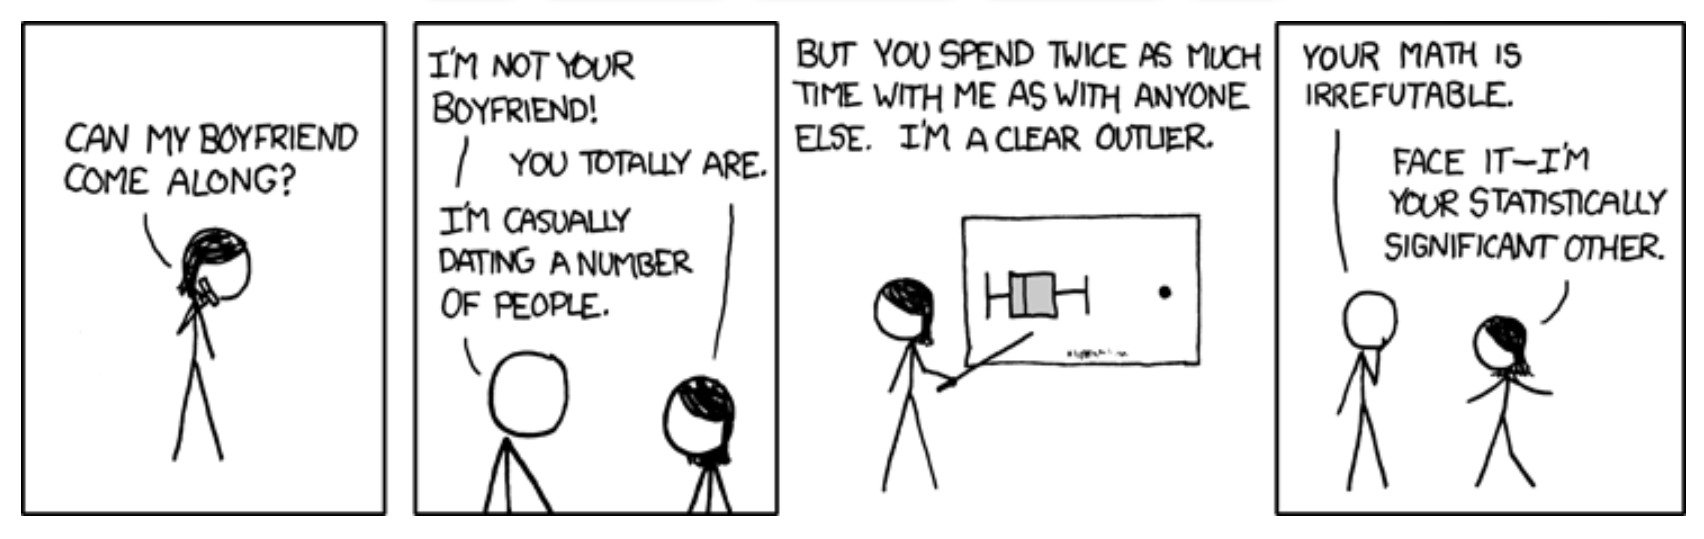
\includegraphics[width=0.7\linewidth]{./images/boyfriend} \end{center}
\end{frame}

\end{document}
